%In den Grundlagen wird das Ziel aller Rahmenwerke, die serviceorientierte Architektur, vorgestellt. Im Anschluss werden alle Rahmenwerke vorgestellt und wichtige Begriffe definiert. Im Hauptteil werden die Kernpunkte des BIAN beleuchtet und mit den äquivalenten Schritten der anderen Rahmenwerke verknüpft. Dabei werden die wesentlichen Unterschiede herausgestellt und bewertet. Im Anschluss werden Verbesserungsvorschläge für die ASAP Methodik gegeben und ein kritisches Fazit gezogen.

\chapter{Grundlagen}

 %   Faktoren zur Messung von Softwarequalität anhand der ISO 9126 vorgestellt und deren Relevanz für diese Bachelorarbeit werden bewertet.

 %   Im Kapitel Grundlagen wird das Konzept der agilen Softwareprogrammierung aufgezeigt und im Nachgang einige ausgewählte Methoden vorgestellt. Aus diesen wird eine Methode ausgewählt, die im Rahmen dieser Bachelorarbeit als Beispiel genutzt wird. Die Vorgehensweise zur Qualitätssicherung ist gleich.

    Im folgenden Kapitel wird der Begriff der Qualität definiert, um anschließend die Qualitätsmerkmale von Software festzulegen. Diese werden auf Grundlage der allgemein gehaltenen ISO 9126-1 definiert, die die Grundlage zu vielen spezifischeren Qualitätsmodellen darstellt. Von diesen Qualitätsfaktoren wird eine bestimmte Menge ausgewählt, die für die Qualitätsprozesse im Rahmen dieser Bachelorarbeit als Kriterien herangezogen werden.

    Im Anschluss daran wird das Konzept der agilen Softwareentwicklung vorgestellt. Neben der Entstehungsgeschichte und den Vor- bzw. Nachteilen der agilen Entwicklung werden verschiedene Vorgehensweisen vorgestellt.

    Daraufhin wird mit den Qualitätssicherungssystemen ebenso verfahren.

    Die Methodiken werden im darauf folgenden Kapitel verglichen und bewertet.

%----------------------------------
%
% Definition von Qualität
%
%----------------------------------
    \section{Definition von Qualität}

        Da der Begriff Qualität im Alltag häufig und in verschiedenen Situationen verwendet wird, soll hier eine Grunddefinition des Qualitätsbegriffs gegeben werden, der im Rahmen der vorliegenden Bachelorarbeit verwendet wird.

        Es kann gesagt werden, \enquote{dass Qualität
            \begin{itemize}
                \item eine Menge von Eigenschaften repräsentiert, die einem Produkt oder Verfahren immanent oder beigegeben ist.
                \item einer der Maßstäbe ist, mit dem der Kunde seine Kaufentscheidung herbeiführt.
                \item ein Faktor ist, der in intensiver Wechselwirkung mit der Wettbewerbssituation und Leistungsfähigkeit eines Anbieters steht.
            \end{itemize}
            \footnote{Pfeifer, 1990.}}

        Dies verfeinert die Definition der ISO 9000: \enquote{Qualität ist der Grad, in dem ein Satz inhärenter Merkmale Forderungen erfüllt\footnote{ISO 90003, 2008, S..}.} Für Qualität bedeutet das, dass einem Werksstück, Prozess oder auch einer Software messbare und nicht messbare Eigenschaften inne wohnen. Bei Software unterscheidet man beispielsweise zwischen messbaren, funktionalen Anforderungen und nicht messbaren, nicht funktionalen Anforderungen. Ein Beispiel für eine funktionale Anforderung ist die Antwortzeit eines Programms, während ein \enquote{gutes} User Interface einer nicht funktionalen Anforderung entspricht. Inhärent sind Merkmale, die sich nach Auslieferung nur sehr schwer oder gar nicht verändern lassen, während der Preis als Beispiel für ein nicht-inhärentes Merkmal sehr frei zu gestalten ist.

        Ein wichtiges Merkmal der vorangehenden Definition ist allerdings die Qualität als Merkmal der Kundenbeeinflussung. Dabei stellt sie sich als Merkmal dar, dass für oder auch gegen die Kaufentscheidung eines bestimmten Produktes spricht. Als Hersteller ist somit eine Sicherung der Qualität unumgänglich um nachhaltig am Markt zu agieren.

%----------------------------------
%
% Qualitätsmerkmale von Software
%
%----------------------------------
    \section{Qualitätsmerkmale von Software}

        Nachdem Qualität als wichtiges Merkmal zum Bilden und Fortbestehen eines Unternehmens identifiziert wurde gilt es nun die Qualität messbar zu machen.

        Die ISO 9126 stellt hierzu sechs Charakteristiken bereit, auf deren Grundlage die Qualität von Software bewertet werden kann. Diese sind in 27 Unterdimensionen unterteilt auf die in den einzelnen Unterpunkten eingegangen wird.
        %Außerdem stellt die ISO 9126 Maßstäbe bereit, um die Unterkategorien zu messen und anhand derer die Erfüllung der Charakteristiken zu bewerten.

        Betrachtet werden nachfolgend die Oberpunkte mit einer Definition nach ISO 9126 und einer Erläuterung. Die ISO Definitionen der Unterkategorien befinden sich im Glossar. Im Anschluss werden drei Merkmale gewählt, die im Rahmen dieser Arbeit betrachtet werden.

    \subsection{Vorstellung der Qualitätsmerkmale}

        Die folgenden Zitate und Absätze orientieren sich vollständig an der ISO 9126-1 Richtlinie.

        \subsubsection{Funktionalität}

            \begin{quote}
              The capability of the software product to provide functions which meet stated and implied needs when the software is used under specified conditions\footnote{ISO 9126-1, 2000, S.7.}.
            \end{quote}

            Die Charakteristik Funktionalität gibt die Fähigkeiten der Software an. Beispielsweise ist eine Funktionalität einer Buchhaltungssoftware die Berechnung einer Gewinn- und Verlustrechnung. Im Gegensatz zu den folgenden Charakteristiken gibt diese an, was die Software tut, statt zu sagen auf welche Weise sie etwas tut.

            Darunter fallen die Abdeckung der gestellten Anforderungen an Funktionalität und Genauigkeit, sowie Sicherheitsaspekte. Im Falle der SAP hat ein Softwareprodukt beispielsweise die Funktion der Geschäftspartnerverwaltung und sollte somit alle fachlich an sie gestellten Anforderungen bedienen. Außerdem sollte bei einer identischen Eingabe stets ein identisches, erwartetes Resultat entstehen. Durch den Scope der zu Beginn eines Projektes erstellt wird ist diese Charakteristik meist schon zu Beginn eines Projekts genau spezifiziert.

            Kunden kaufen Software in der Annahme, dass diese einen Mehrwert für diesen darstellt. Das bedeutet, dass die Software die Arbeit des Kunden erleichtert oder die Qualität seiner Arbeit erhöht. Damit ein Mehrwert geschaffen werden kann müssen die versprochenen Funktionen abgedeckt sein. Eine Software zur Verwaltung von Geschäftspartnern würde keinen Mehrwert liefern, wenn es nicht möglich wäre neue Geschäftspartner anzulegen.


        \subsubsection{Verlässlichkeit}

            \begin{quote}
              The capability of the software product to maintain a specified level of performance when used under specified conditions\footnote{ISO 9126-1, 2000, S.8.}.
            \end{quote}

            Die Charakteristik Verlässlichkeit gibt die Fähigkeit einer Software an unter den festgelegten Rahmenbedingungen immer in einem vorher festgelegten Rahmen zu reagieren. In alten Definitionen bezog sich die Verlässlichkeit darauf eine bestimmte, benötigte Funktion auszuführen.

            Das Ziel ist eine Software, die zu jederzeit in dem erwarteten Umfang reagiert und falsche Eingaben, falsche Benutzungsweisen und ungültige Datensätze verkraftet oder verhindert. Software ist genau dann verlässlich, wenn keine Fehler durch Defekte in der Software auftreten, keine Angriffe, bewusst oder unbewusst, von außen oder innen möglich sind und sämtliche Daten auch nach einem Systemabsturz wieder herstellbar sind.

            Unternehmen der Finanzindustrie besitzen häufig Softwarelandschaften, die in den 1970er Jahren aufgebaut werden und seitdem im Stand gehalten und erweitert werden.\footnote{Vgl. TOGAF/Bian, 2013, S.10.} Die auf Mainframes aufgebauten Architekturen sind sehr teuer in Wartung und Entstandhaltung, aber gewährleisten eine hohe Erreichbarkeit von bis zu 99.999\%. Dies bedeutet, dass ein Mainframe nur circa 5,26 Minuten pro Jahr nicht zu erreichen ist. IBM gibt für ihre Mainframes zudem eine durchschnittliche Zeit zwischen Fehlern von 20 bis 30 Jahren an. Außerdem werden Operationen häufig mehrfach gleichzeitig durchgeführt und die Ergebnisse verglichen. Somit sind fehlerhafte Berechnungen nahezu ausgeschlossen.\footnote{Symonds, 2013, S.12.} Unternehmen der Finanzindustrie stellen somit hohe Anforderungen an ihre IT Systeme und die zuverlässige Ausführung von Prozessen ist bei der Verarbeitung von Zahlungsströmen u.ä. unverzichtbar.

        \subsubsection{Benutzerfreundlichkeit}

            \begin{quote}
              The capability of the software product to be understood, learned, used and attractive to the user, when used under specified conditions\footnote{ISO 9126-1, 2000, S.9.}.
            \end{quote}

            Benutzbarkeit sagt aus, dass ein fachlich versierter Anwender intuitiv die Funktion des Programms erkennt und es verwenden kann. Dabei soll der Anwender nach Möglichkeit ein gutes Gefühl haben und die Software als schön bezeichnen.

            Das Ziel der SAP ist es durch eine intuitive Menüführung beim Endbenutzer einen Produktivitätszuwachs zu erreichen, indem dieser schnell und sicher durch die Oberfläche navigieren kann. Durch leicht zu verstehende Oberflächen soll zudem die zur Einarbeitung benötigte Zeit reduziert werden. Somit wird im Idealfall der Schulungsbedarf des Kunden reduziert.

            Aus dem Privatleben sind geschäftliche Anwender inzwischen einfache, intuitive Oberflächen gewöhnt und tragen diese als Anforderung ins Unternehmen. Außerdem werden mehr mobile Geräte in Unternehmen verwendet. Um alle Daten, zu jeder Zeit und an jedem Ort zur Verfügung zu haben werden die Daten häufig in der Cloud bereitgestellt und über webbasierte Applikationen angezeigt. SAP verfolgt mit dem Paradigma Fiori die Strategie, dass sich die Oberflächen zwischen mobilen Geräten und Computern nicht unterscheiden und keine Daten auf dem Gerät liegen. Durch einheitliche Oberflächen soll die Produktivität der Nutzer erhöht werden und die Einarbeitungszeit reduziert werden.

        \subsubsection{Effizienz}

            \begin{quote}
              The capability of the software product to provide appropriate performance, relative to the amount of resources used, under stated conditions.
            \end{quote}

            Der Faktor Effizienz drückt das Verhältnis zwischen der Performance der Software und den dafür verbrauchten Ressourcen aus. Die Effizienz steigt, wenn die Performance bei gleichbleibendem Ressourcenverbrauch steigt oder wenn bei gleichbleibender Performance der Ressourcenverbrauch sinkt und umgekehrt.

            Um selbst bei umfangreichen Datenabfragen und Berechnungen eine geringe Antwortzeit zu gewährleisten verfolgt SAP den Trend der In-Memory Datenhaltung. SAP verwendet hierzu die SAP High Performance Analytical Appliance (HANA). Trotz der gestiegenen Ressourcennutzung ist der Performance Gewinn größer um deren Verwendung zu rechtfertigen. Gerade im Umgang mit Massendaten, die im Finanzbereich anfallen ist eine effiziente Datenhaltung und Verarbeitung sehr empfehlenswert.

        \subsubsection{Wartbarkeit}

            \begin{quote}
              The capability of the software product to be modified. Modifications may include corrections, improvements or adaptation of the software to changes in environment, and in requirements and functional specification.
            \end{quote}

            Die Wartbarkeit einer Software wird anhand der Möglichkeit bewertet Korrekturen, Verbesserungen und neue Funktionen einzuspielen. Außerdem sollte die Software an neue Anforderungen, wie neue Prozesse oder neue Umsysteme anpassbar sein.

            Eine stetige Zunahme an regulatorischen Anforderungen in einem dynamischen Marktumfeld erfordern flexible und modulare Systeme. Da kein allumfassendes Softwareprodukt pro Branche bereit gestellt werden kann müssen die Systeme in ihre Umgebung, insbesonde historisch gewachsene, bestehende Systeme, eingegliedert werden.

        \subsubsection{Portierbarkeit}

            \begin{quote}
              The capability of the software product to be transferred from one environment to another.
            \end{quote}

            Die Portierbarkeit der Software ist besonders hoch, wenn sie so universell programmiert ist, dass sie ohne oder mit minimalem Aufwand auf verschiedenen Infrastruktur und Software Plattformen verwendet werden kann. Für SAP als Anbieter von Standardsoftware ist dies einer der Hauptfaktoren zur Entwicklung von Software, da dies die Grundlage zur Wiederverwendung von entwickelten Softwarebausteinen bildet.

        \subsection{Auswahl und Bewertung der Qualitätsmerkmale}

            Funktionalität bewertet den Funktionsumfang der Software. Wenn die Software nicht alle wichtigen Anforderungen des Kunden erfüllt ist die Investition in diese Software nicht gewinnbringend und er wird sie nicht tätigen. Daher wird die Funktionalität als erstes Bewertungskriterium in dieser Arbeit herangezogen.

            Die korrekte und vollständige Ausführung von Operationen auf der Software ist für Unternehmen der Finanzdienstleistungsindustrie sehr wichtig, da Kunden einen hohen Standard gewohnt sind und Fehler sehr kostspielig sein können. Es ist daher essentiell, dass die Software verlässlich arbeitet, korrekte Ausgaben erzeugt und die Daten sicher hält. Verlässlichkeit wird daher auch als Bewertungskriterium in dieser Arbeit herangezogen.

            Benutzerfreundlichkeit wird hauptsächlich durch die Anwendungsoberfläche bestimmt. Die Implementierung von Software ermöglicht es zudem die Anwendungsoberfläche unabhängig von der Datenhaltung und der Datenverarbeitung zu erstellen in einer so genannten 3-Schichten-Architektur. Da die Endanwender häufig nicht die Käufer einer Software sind und für SAP durch reduzierten Schulungsbedarf kein unmittelbarer Mehrwert entsteht ist eine intuitive und selbsterklärende Oberfläche nicht kritisch für den Verkauf von Software und einer Zufriedenstellung des Kunden. Die Benutzerfreundlichkeit der Software wird im Rahmen dieser Arbeit außen vor gelassen.

            Bausparverträge und Baufinanzierungen sind meist langfristig orientierte Verträge und werden nach einer umfassenden Beratung und im idealfall auch nach einem Vergleich von Angeboten angelegt und unterschrieben. Das bedeutet, dass innerhalb dieses Geschäftszweigs keine Echtzeitdaten benötigt werden, sondern eine zeitnahe Beantwortung von Anfragen ausreicht. Für die Effizienz bedeutet dies, dass mit einem vertretbaren Aufwand vertretbare Resultate erzeugt werden sollen, ohne das technische Grenzen ausgereizt werden müssen. Effizienz ist daher kein Teil der in dieser Arbeit betrachteten Kriterien.

            Die Finanzindustrie untersteht einem stetigen, disruptiven Wandel, der durch neue regulatorische Anforderungen und neue Konkurrenzen, sogenannte Fin-Techts, verursacht wird. Die neuen Marktteilnehmer bauen ihre IT ohne störende Altlasten auf und können so dynamisch auf das Marktumfeld reagieren. Um auch die eigene Software zukunftsfähig zu machen und selbst konkurrenzfähig zu bleiben muss eine Unternehmensplattform anpassbar und flexibel sein. Eine leicht zu wartende Lösung reduziert die Betriebskosten und bildet die Grundlage zur zukunftsfähigen IT. Wartbarkeit ist daher ein wichtiges Kriterium und bidet somit das letzte Kriterium, dass im Rahmen dieser Arbeit verwendet wird.

            Da SAP als reiner Softwarehersteller keine Hardware verkauft muss SAP Software auf verschiedenen Platformen und Betriebssystemen anwendbar sein. Da SAP Instanzen in eigenen Laufzeitumgebungen auf dem Betriebssystem laufen ist die Kompabilität der Software mit verschiedenen Betriebssystemen keine Aufgabe der Entwickler für Geschäftsanwendungen. Diese Charakteristik ist daher ebenso zu vernachlässigen.

            Im Folgenden wird daher für den Entwicklungsprozess eine funktionale, verlässliche und wartbare Software als Ziel festgesetzt.

%----------------------------------
%
% Agile Methoden
%
%----------------------------------
    \section{Agile Methoden}

        \begin{quote}
          Achieving a product which satisfies the user's needs normally requires an iterative approach to software development with continual feedback from a user perspective.\footnote{ISO 9126-1, 2000, S.4.}
        \end{quote}

        Agile Methoden wurden mit dem Ziel entwickelt den Endbenutzer früher in die Softwareentwicklung einzubeziehen, um ein Produkt zu entwerfen, dass tatsächlich benötigt wird. Hierzu werden möglichst schnell und möglichst viele einzelne, aber lauffähige Code-Fragmente entwickelt, die dem Kunden vorgeführt werden um diesen ein Gefühl für die Software zu geben. Das frühe Feedback des Kunden ermöglicht es schon früh während des Entwicklungsprojekts Anpassungen vorzunehmen um die realen Bedürfnisse zu erfüllen.

        Hierzu wurden Prinzipien entwickelt, die einfach und granular die Idee der agilen Entwicklung herunterbrechen. Diese wurden im agilen Manifest festgehalten und verbreitet. Hierbei ist zu beachten, dass jeweils nicht nur der erste Teil der Prinzipien beachtet werden soll, sondern dieser eine höhere Gewichtung zukommt.\footnote{Vgl. Agile Manifesto, 2015.}

        \subsection{Prinzipien der agilen Entwicklung}

            \subsubsection{Individuals and interactions over processes and tools}

                Software Entwicklung wurde vor den agilen Entwicklungsmethoden sehr weit standardisiert und geplant\footnote{Vgl. Schneider, 2007, S..}. Hierdurch waren die Entwickler häufig sehr unflexibel und konnten nicht auf Wünsche oder Anpassungsvorschläge reagieren, sobald diese den Zeitplan verletzt hätten.

                Um dieser Entwicklung entgegenzuwirken stellt das agile Manifest die Interaktion mit dem Kunden und unter den Entwicklern an erste Stelle, anstatt das diese von Prozessen regiert werden.

                Ein reger Austausch soll gefördert und auf die Bedürfnisse der einzelnen Personen soll eingegangen werden.

            \subsubsection{Working software over comprehensive documentation}

                Durch viel bürokratischen Aufwand und eine umfangreiche Planung von Software wird zu Beginn des Projektes sehr viel Aufwand investiert ohne einen konkreten Mehrwert gegenüber stehen zu haben. Durch die dynamische Grundhaltung bei der agilen Entwicklung wird zu Beginn sehr wenig Zeit in die Planung investiert, die Entwicklung kann direkt gestartet werden und schon nach kurzer Zeit gibt es lauffähige Programmbestandteile.

                Dieses Prinzip drückt aus, dass am Ende eines Projekts eine lauffähige Software, die die Ansprüche des Kunden erfüllt einer umfangreichen Dokumentation mit unvollständiger Software zu bevorzugen ist.

            \subsubsection{Customer collaboration over contract negotiation}

                SAP hat als Hersteller von Standardsoftware zur Unternehmenssteuerung das Ziel Software zu entwickeln und diese zu verkaufen. Der Verkauf von Software wird erheblich erleichtert, wenn diese ein Bedürfnis des Kunden erfüllt und bei diesem die tägliche Arbeit erheblich vereinfacht.

                Um die Anforderungen des Kunden zu verstehen und bei der Entwicklung der Software zu berücksichtigen sollte dieser schon früh einbezogen werden. Die agilen Methoden sollen dabei auf die Wünsche des Kunden reagieren, statt jede Abweichung eines aufgestellten Plans mit umfangreichem bürokratischen Aufwand zu verhandeln.

            \subsubsection{Responding to change over following a plan}

                Insbesondere bei längeren Projekten ist es meist absurd anzunehmen, dass man die Anforderungen des Unternehmens in ferner Zukunft kennt. Bei Unternehmen der Finanzindustrie werden häufig neue regulatorische Anforderungen veröffentlicht oder das Marktumfeld verändert sich. Um auf diese Änderungen auch während der Projektlaufzeit eingehen zu können und keine zum Release veraltete Software einzusetzen sollte im Projekt auf Veränderungen eingegangen werden.

        \subsection{Ausgewählte Methoden der agilen Entwicklung}

            Im Folgenden werden konkrete herangehensweisen zur agilen Entwicklung vorgestellt. Diese sind genau wie die Prinzipien des agilen Manifests sehr allgemein und locker gehalten um den Entwicklern hinreichend Freiraum zu geben um Ideen ausleben zu können. Dies entspricht der Idee der agilen Entwicklung.

            \subsubsection{Lean Software Development}

                Die Grundlage des Lean Software Developments bildet der Produktentwicklungsprozess von Toyota. Im Anschluss an den zweiten Weltkrieg wurde dort die Automobilproduktion aufgebaut und da in Japan weder der Platz noch die Ressourcen vorhanden waren um die ineffiziente amerikanische Automobilproduktion zu immitieren wurden neue Prinzipien in die Entwicklung integriert, die die Lagerhaltung, Massenfertigung und Produktentwicklung betreffen.\footnote{Vgl. Dombrowski, 2015, S.7.} Der Entwicklungsprozess baut auf sieben Prinzipien auf, die zusammen mit agilen Methoden auch auf die Softwareentwicklung angewendet werden können.

                Die bisherige Annahme im Produktentwicklungsprozess, unabhängig von Software, Autos o.ä., war, dass ein Fehler, der während der Planung eliminiert wird um den Faktor 1000 günstiger ist als ein Fehler, der beim Kunden entdeckt wird. Dies leitet sich aus der so genannten Zehnerregel der Fehlerkosten ab:

                \begin{figure}[!htbp]
                        \begin{center}
                        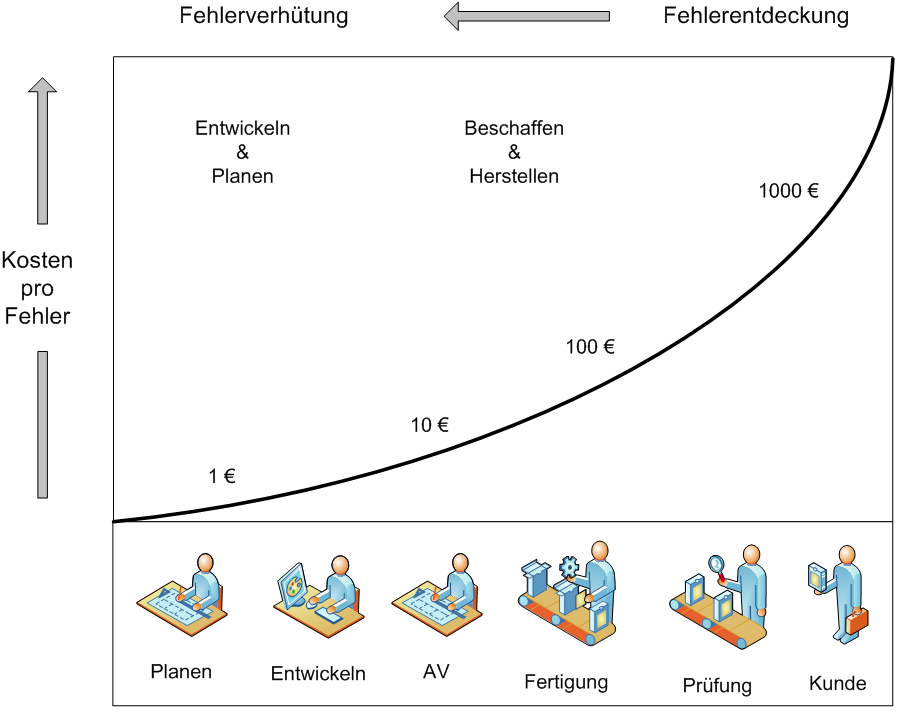
\includegraphics[width=11cm]{Abbildungen/zehnerregel}
                        \caption{Zehnerregel der Fehlerkosten\protect\footnotemark}
                        \label{abb:zehnerregel}
                        \end{center}
                \end{figure}

                \footnotetext{http://www.sixsigmablackbelt.de/fehlerkosten-10er-regel-zehnerregel-rule-of-ten/}

                Im Rahmen von Lean Development halten sich die praktizierenden Unternehmen während des Designprozesses jedoch möglichst viele Optionen offen, um während des Produktionsprozesses Entscheidungen auf einer optimalen Faktenbasis zu treffen und nicht durch plausible Annahmen.\footnote{Vgl. Poppendieck, 2003, S.5.} Solche Design- und Funktionsentscheidungen sehr spät im Prozess zu treffen wird beispielsweise in Scrum praktiziert, indem erst zu Beginn jedes Sprints die Anforderung des Kunden festgelegt wird und nicht in einem umfangreichen Scopedokument zu Beginn des gesamten Projektes.

                Die Prinzipien des Lean Developments lassen sich als agilen Prozess anwenden oder auf agile Prozesse ummünzen. Folgende Prinzipein wurden als Kern des Lean Development identifiziert\footnote{Poppendieck, 2003, S. 13.}:

                \begin{itemize}
                  \item Eliminate waste
                  \item Amplify learning
                  \item Decide as late as possible
                  \item Deliver as fast as possible
                  \item Empower the team
                  \item Build integrity in
                  \item See the whole
                \end{itemize}

                Im folgenden wird eine kurze Einführung der Unterpunkte gegeben mit einer Erläuterung, wie sie als agiler Prozess aufzusetzen sind.

                \enquote{Waste is anything that does not add value to a product, value as perceived by the customer.}\footnote{Poppendieck, 2003, S.13.} Dies umfasst bezogen auf die Softwareentwicklung nicht nur sämtliche Applikationen, die nicht benötigt werden, sondern auch ungenutzte Funktionen und das potenzial zu möglichen, zukünftigen Erweiterungen im Code. Das Ziel sollte es sein den Code so klein wie möglich zu halten um die unmittelbaren Bedürfnisse des Kunden zu befriedigen. Das bedeutet, dass in jeder Iteration des Entwicklungsprozesses nur die Funktion entwickelt wird, die der Anwender braucht und die am höchsten priorisiert ist. Rein statistisch werden etwa 50\% aller Funktionen einer Software selten oder nie genutzt\footnote{Ebert, 2007} Wenn dieser Überschuss eliminiert wird werden die Programme schlanker, einfacher und günstiger in der Wartung, ohne das der Anwender auf wichtige Funktionen verzichten muss.

                Die Entwicklung eines Produktes ist im Gegensatz zur Herstellung eines Produktes kein linearer Prozess, der vorher skizziert und abgearbeitet werden kann. Obwohl Variation in der Produktion reduziert beziehungsweise eliminiert werden soll ist sie im Entstehungsprozess eines Produkts durchaus wünschenswert, um die bestmögliche Lösung zu finden.\footnote{Vgl. Ballard, 2000, S. 2f.} Um möglichst viele Optionen zu betrachten und sich mit fortgeschrittenem Kenntnisstand für eine zu entscheiden hat Toyota das so genannte \emph{Set-Based Concurrent Engineering} entwickelt, bei dem mehrere Prototypen in die Entwicklung mitgeführt werden, statt zu Entwicklungsbeginn einen Designstop einzulegen. Diese Protoypen werden mit dem jeweils aktuellen Kenntnisstand weiterentwickelt und eine Entscheidung zu Gunsten einer Variante fällt so spät wie möglich. Zur Entwicklung dieser Methoden wird ein Prozess von drei Oberpunkten vorgesehen, die die Menge von Möglichkeiten filtern:

                \begin{itemize}
                  \item Map the design space
                  \item Integrate by intersection
                  \item Establish feasibility before commitment\footnote{Sobek, 2000, S.73.}
                \end{itemize}

                Zunächst wird daher der Rahmen festgelegt, in dem entwickelt werden darf. Dies betrifft übertragen auf die Softwareentwicklung Programmiersprachen und Systeme. Im Anschluss werden Konzepte in diesem Rahmen übereinandergelegt und die Variation auf das nötigste reduziert. Abschließend werden alle verbliebenen Vorgehensweisen auf Machbarkeit geprüft und auf Basis dieses Ergebnisses eine Entscheidung getroffen. Die Reduzierung der Grenzen bis zur Entscheidung für eine Vorgehensweise lernen die Entwickler aus dem Entwicklungsprozess und die Möglichkeit, die den größten Nutzen bietet wird umgesetzt.
                Dies ist auch der Grund dafür, dass eine möglichst späte Entscheidung angestrebt wird.

                Die Vorgabe so schnell wie möglich Ergebnisse zu liefern bedeutet nicht, dass ein unfertiges oder unreifes Produkt ausgeliefert werden soll, sondern das lauffähige Versionen entstehen, auf deren Grundlage die Entwicklung voranschreiten kann. Somit kann ein Kunde herausfinden was er benötigt und die Richtung des Projektes besser gesteuert werden. Dies führt zu kurzen Iterationen, die lauffähige Ergebnisse liefern.

                Der reine Einsatz von Methoden führt häufig nicht zu den gewünschten Ergebnissen. Es geht ebenfalls darum die Mitarbeiter in den Prozess der Produktentstehung einzubinden und alle Ideen und Kompetenzen zu nutzen. Bisherige Softwareentwicklungsprozesse zielen darauf ab zu Beginn der Entwicklung Entscheidungen von einer Hand voll Personen zu treffen, die die tatsächliche Implementierung meist nicht persönlich umsetzen. In einem Lean Development Umfeld sollen die Entscheidungen von den umsetzenden Personen getroffen werden und die oberen Hierarchien durch Reports, Grafiken und regelmäßige Meetings lediglich informiert werden. Dies beschleunigt Iterationen und ermöglicht mehr Tests und Versuche, die zu besseren Ergebnissen führen.\footnote{Vgl. Poppendieck, 2003, S.14}

                Die Integrität einer Software wird daran gemessen, wie zufrieden jemand ist, der mit dieser Software arbeitet, unabhängig davon ob eben dieser Anwender oder Entwickler ist. Hierbei beruft sich Poppendieck auf die Qualitätskriterien von Software der ISO 9126-1, die oben vorgestellt wurden. Sie sagt, dass dies nicht durch Prozesse und Messungen umsetzbar sei, sondern durch weise Führung, fachliche Expertise, effiziente Kommunikation und gesunde Disziplin.\footnote{Vgl. Poppendieck, 2003, S.14.} Der Weg zur Integrität einer Software basiert daher auch auf einigen Prinzipien des agilen Manifests.

                Zuletzt soll das Gesamtziel des Projektes nicht aus den Augen verloren werden. Die absolute Optimierung eines Teilbereichs zu Lasten des Gesamtprojekts sollte zwingend vermieden werden.

                Zusammenfassend ist Lean Software Development eine Menge von Prinzipien, die aus der Entwicklung von Autos abgeleitet wurde und zu Beginn eines Projektes als konkrete Pläne umgesetzt werden sollen. Wie die im Folgenden vorgestellten agilen Programme weißt es auf typische Fehler hin und gibt Ratschläge, wie sie vermieden werden können, ohne die Freiheit des Teams einzuschränken.

            \subsubsection{Extreme Programming}

                \begin{quote}
                  XP is a style of software development focusing on excellent application of programming techniques, clear communication, and teamwork which allows us to accomplish things we previously could not even imagine.\footnote{Andres, 2005, S..}
                \end{quote}

                \enquote{Extreme Programming ist eine leichtgewichtige Softwareentwicktlungs-Methode, mit einem Wertesystem sowie einer Sammlung von Grundprinzipien und Entwicklungspraktiken\footnote{Rumpe, 2001, S..}.}
                Extreme Programming räumt mit einigen Konventionen der Softwareentwicklung auf, indem es die bisher bestehenden Prozesse bewusst kritisiert und eigene Werte und Modelle präsentiert, die die Softwareentwicklung vereinfachen.

                Extreme Programming orientiert sich dennoch an einem groben Prozess zur Entwicklung von Software. Zunächst wird eine User Story entworfen, das heißt ein Anwender beschreibt was er tun muss und an welchen Stellen er dabei unterstützt werden müsste. Zur Erläuterung des Prozesses wird nachfolgend das Anlegen eines Vertrags in einer Filiale aus Sicht eines Angestellten betrachtet.

                Der Anwender möchte die Daten des Kunden in die Softwareoberfläche eintragen und anschließend einen Vertrag mit den Konditionen für diesen Kunden ausdrucken. Die Daten sollen zudem in der Datenbank der Bausparkasse hinterlegt werden. Daraus ergibt sich eine neue Aufgabe für die Softwareentwickler.

                Extreme Programming sieht vor, dass für jede zu entwickelnde Komponente zunächst ein Test geschrieben wird. Die Tests bilden das pendant zur klassischen Spezifikation und werden nach jeder Änderung der Software überprüft um so eine ständige Lauffähigkeit des Moduls zu gewährleisten. Ein Test würde beispielsweise prüfen, wie mit unvollständigen Angaben umgegangen wird und wenn kein Drucker erreichbar wäre. Bei der Erstellung der Test-Fälle sollten alle gewöhnlichen Eingaben, ungültige Eingaben und Randwerte, wie zum Beispiel unendlich große bzw. unendlich kleine Bausparsummen geprüft werden.\footnote{ANGABE SUCHEN}

                Auf Grundlage der entworfenen Tests startet die Entwicklung, die die Ansprüche des Anwenders, die im Test formalisiert wurden, erfüllen soll. Im Gegensatz zur klassischen Entwicklung von Software, bei der jeder Entwickler für einen Baustein das Programms zuständig ist und diesen in Einzelarbeit vorantreibt wird im Extreme Programming Pairprogramming empfohlen. Außerdem sollen alle Entwickler jederzeit den gesamten Code kennen und dürfen an jeder Stelle etwas verändern, sobald sie Fehler entdecken. Das Ziel ist es die Abhängigkeit von einzelnen Entwicklern zu reduzieren und schon während der Entwicklung eine ständige Kontrolle durch den Partner zu haben. Studien haben außerdem nachgewiesen, dass zwei Entwickler die Entwicklungszeit reduzieren und weniger Fehler produzieren\footnote{ANGABE SUCHEN}.

                \begin{figure}[!htbp]
                    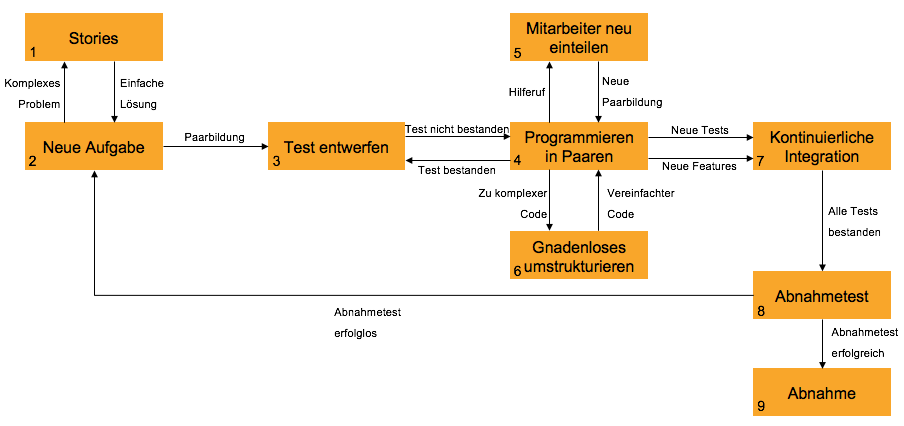
\includegraphics[width=15cm]{Abbildungen/XP_vorgehensmodell}
                    \caption{Vorgehensmodell des Extreme Programming\protect\footnotemark}
                    \label{abb:xpmodel}
                \end{figure}

                \footnotetext{https://www.st.cs.uni-saarland.de/edu/lehrer/xp.pdf, 2016.}

                Extreme Programming hat darüber hinausgehend noch zwei Prinzipien, die bei der klassischen Softwareentwicklung in dieser Form nicht angewendet werden. Zunächst wird immer nur ein aktuelles Problem gelöst und es werden keine Pläne für zukünftige Integrationen und Erweiterungen im Code umgesetzt. Der Code soll so einfach wie möglich gehalten werden und die Voraussetzung ist, dass ein einfacher Code später besser anzupassen ist, als komplizierten Code mit einer Schnittstelle zu haben, die eventuell nie gebraucht wird.

                Das zweite Prinzip ist der selbstdokumentierende Code. Über sprechende Methodennamen und Kommentare soll jeder Entwickler zu jeder Zeit verstehen, was sich der Autor des Codes gedacht hat. Dieser sprechende Code soll die Dokumentation der Software obsolet machen. Dies geschieht aus dem Grund, dass Dokumentationen häufig nicht aktuell sind oder nicht mit dem gleichen Eifer wie der Code entwickelt wurden und somit fachlich falsch sind. Diese Ziele werden erreicht, indem sehr viele Kommentare verwendet werden und das bisher entwickelte \emph{Refactored} wird. Das bedeutet, dass Codebruchstücke, wie beispielsweise eine Tabellenabfrage in eine Methode ausgegliedert werden und stattdessen die Methode im Hauptprogramm aufgerufen wird. Diese ständigen Restrukturierungen vereinfachen das bisher entwickelte und lassen den Umfang des Programms nicht ausufern.

                Natürlich stößt aber auch das Extreme Programming in Projekten an Grenzen. Die Pairprogramming Methodiken setzen voraus, dass die Entwickler auf engem Raum zusammen arbeiten und nicht allzu weit verstreut sind. Außerdem muss für die ständige Abstimmung und Kommunikation das Team sehr klein gehalten werden, meist werden 9-12 Personen empfohlen.

                Extreme Programming stellt konkrete Anforderungen an das Team und lässt in der Umsetzung die wenigsten Freiheiten der agilen Methoden. Es ist, wie der Name impliziert, eine sehr extreme Herangehensweise, die Tests, Entwicklung und Flexibilität maximiert. Häufig können jedoch vereinzelte Methoden des Extreme Programming in anderen agilen Verfahren verwendet werden um ein Teil von methodischer Flexibilität zu erhalten.

            \subsubsection{Scrum}

                  Scrum ist ein \enquote{Ein Rahmenwerk, innerhalb dessen Menschen komplexe adaptive Aufgabenstellungen angehen können, und durch das sie in die Lage versetzt werden, produktiv und kreativ Produkte mit dem höchstmöglichen Wert auszuliefern.} Es ist
                  \begin{itemize}
                      \item Leichtgewichtig
                      \item Einfach zu verstehen
                      \item Schwierig zu meistern.\footnote{Scrum Guide, 2013, S..}
                  \end{itemize}

                  Im Gegensatz zum Extreme Programming ist Scrum ein Rahmenwerk statt einer Methode, dass neben konkreten Managementvorgaben sehr viel Gestaltungsfreiraum bietet. Scrum setzt auf einen iterativen, inkrementellen Ansatz, was bedeutet, dass kurze Phasen der Entwicklung ständig wiederholt werden und das Endprodukt Stück für Stück aufgebaut wird. Mit jeder abgeschlossenen Phase wird die Software um einen weiteren Baustein ergänzt.

                  Für nach Scrum organisierte Teams wird eine Personenanzahl von 5-9 Entwicklern zuzüglich Scrum Master und Product Owner empfohlen. Somit soll die Organisation flexibel genug sein um sich selbst koordinieren zu können, aber groß genug um alle notwendigen Kenntnisse abzudecken, sodass das Team während der Softwareentwicklung nicht auf externe Hilfe angewiesen ist. Im Folgenden werden die einzelnen Rollen in der Entwicklung betrachtet:

                  Der Product Owner hat die Verantwortung, dass der Kunde das erhält, was er sich wünscht. Er steht in ständigem Austausch mit eben diesem, präsentiert Zwischenergebnisse und trägt die neuen Wünsche priorisiert in das Entwicklungsteam. Alle Wünsche und Anforderungen, die an das Team gestellt werden haben über den Product Owner zu laufen.

                  Der Scrum Master vertritt die Interessen der Entwickler gegenüber Außenstehenden und dem Product Owner. Er sorgt dafür, dass die Scrum-Regeln eingehalten werden und die Entwickler während ihrer Entwicklungsphasen nicht gestört werden. Der Scrum Master hat keine Weisungsbefugnis inne, sondern versucht einem Ombusmann ähnlich Win-Win Situationen für alle Parteien zu erreichen. Als erfahrenes Scrum-Teammitglied steht er außerdem für alle Fragen zur Verfügung und coached seine Kollegen bei Bedarf.

                  Das Entwicklungsteam setzt sich aus einer Vielzahl von Experten zusammen, die alle benötigten Kompetenzen abdecken. Das gesamte Entwicklungsteam ist verantwortlich für den gesamten Code und organisiert sich vollständig selber.\footnote{Vgl. Scrum Guide, 2013, S..}

                  Neben dem Team umfasst Scrum auch Vorgaben zum Ablauf. Hierfür werden eine Menge von Meetings und Phasen vorgegeben, die einen festen Zeitraum haben, der nicht überschritten werden darf. Auf Grundlage dieser Annahmen sind Scrum-Projekte sehr planbar.

                \enquote{Das Herz von Scrum ist der Sprint, eine Time Box von maximal einem Monat, innerhalb dessen ein fertiges (\emph{Done}), nutzbares und potenziell auslieferbares Produkt-Inkrement hergestellt wird}\footnote{Scrum Guide, 2013, S.8.}. Dies entspricht der oben bereits vorgestellten Entstehung von Software durch Bausteine, die ein Grundkonstrukt um Funktionen erweitern. Wichtig ist dabei, dass jeder Baustein fertig ist, was durch den Ausdruck Done im Zitat versinnbildlicht wird. Die Definition von Done sollten von Product Owner, Scrum-Team und Kunde vorab festgelegt und festgehalten werden, damit es dort zu keinen Missverständnissen kommt.

                Ein Sprint dauert für gewöhnlich vier Wochen und beinhaltet eine Menge von Ereignissen:
                  \begin{itemize}
                    \item Sprint Planning
                    \item Daily Scrums
                    \item Sprint Review
                    \item Sprint Retrospektive
                  \end{itemize}

                  \begin{figure}[!htbp]
                        \begin{center}
                        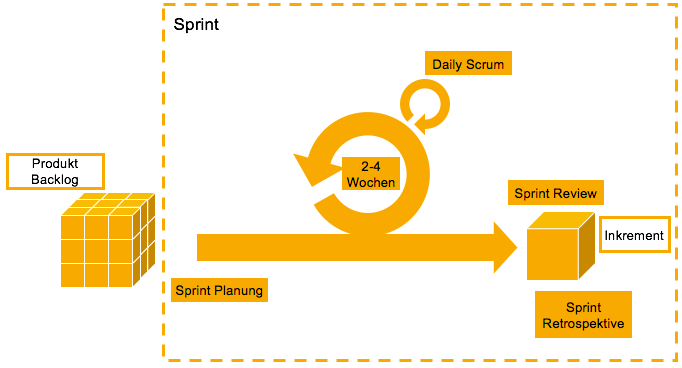
\includegraphics[width=11cm]{Abbildungen/scrum}
                        \caption{Planungszyklus Scrum\protect\footnotemark}
                        \label{abb:scrum}
                        \end{center}
                  \end{figure}

                  \footnotetext{Eigene Grafik erstellen!}

                Während des Sprint werden keine weiteren Themen zum Scope ergänzt und weder Zeit- noch Qualitätsplanung angepasst. Erst die Sprint-Planung am Ende jedes Zyklus bietet die Möglichkeit zur Nachkalibration. Die Dauer eines Sprints ist daher auch so gewählt, dass das Projekt flexibel genug ist um auf Anforderungen einzugehen, die Entwickler allerdings die Chance erhalten sich voll und ganz auf eine Aufgabe zu konzentrieren und nicht ständig durch Anforderungsänderungen aus ihrem Fokus gerissen werden. Im Folgenden werden die vier Phasen eines Sprints weiter aufgeschlüsselt:

                Das \emph{Sprint Planning} dient als Vorbereitung für den kommenden Sprint. Im Zentrum des Planungsprozesses stehen zwei Fragen, die am Ende des Meetings beantwortet sein sollen.
                \begin{itemize}
                  \item Was kann in diesem Sprint fertiggestellt werden?
                  \item Wie wird die ausgewählte Arbeit erledigt?
                \end{itemize}

                In der ersten Phase präsentiert der Product Owner die Wünsche des Kunden und nennt priorisiert alle Dinge, die bis zum Ende des Sprints geschafft werden sollten. Das Entwicklungsteam diskutiert mit ihm daraufhin, ob die Zeitplanung und Deadlines realistisch sind, oder ob es denkt deutlich mehr bzw. deutlich weniger zu schaffen. Haben sich Product Owner und Scrum Team auf einen Scope geeinigt kommt es zu Phase zwei des Sprint Planning, in der geplant wird, wie das Sprint-Ziel zu erreichen ist.

                Die Vorgehensweise stellt bei Software beispielsweise grob die Codestruktur dar mit Methoden, Eigenschaften von Klassen usw. Sie lässt sich beispielsweise durch UML-Klassendiagramme sehr gut erfassen. Hierbei sollen unabhängig von Kompetenzen und Erfahrungen alle Ideen des Teams eingebracht werden. Ein großes Problem bei Sprint Plannings sind häufig Externe, insbesondere Vorgesetzte, die bei jungen Entwicklerteams oft Ratschläge geben, die aber als Weisung aufgenommen werden. Durch die Präsenz weisungsbefugter Personen wird die Kreativität im Team so häufig untergraben und nicht vollkommen ausgeschöpft.
                Der Scrum Master hat zusätzlich noch die Aufgabe sehr dominante und aktive Personen zu bremsen und auch die ruhigeren Charaktere in die Diskussion mit einzubinden. Während des Sprint Plannings und auch dem gesamten Sprint fungiert er als Moderator.\footnote{Vgl. Maximini, 2013, S.182f.}

                Das \emph{Daily Scrum} findet Arbeitstäglich statt, dauert meist 15 Minuten und ist ein Meeting mit dem gesamten Team. Um Dynamik zu erzeugen und nicht zu überziehen findet es meist im stehen kurz vor der Mittagspause statt. Das Daily Scrum dient dazu dem gesamten Entwicklungsteam eine Übersicht zu geben, wer wo steht und wie weit man als Team bei der Verwirklichung des Sprint Ziels ist. Außerdem findet man häufig eine Lösung, wenn Probleme auftreten und diese im Team vorgestellt werden. Jedes Mitglied des Scrum-Teams ist nacheinander an der Reihe und beantwortet in der großen Runde folgende drei Fragen:

                \begin{itemize}
                  \item Was habe ich gestern getan?
                  \item Was werde ich bis morgen tun?
                  \item Wo bin ich dabei auf Hindernisse gestoßen?
                \end{itemize}

                Insbesondere bei der letzten Frage geht es nicht darum Lösungen während des Daily Scrums zu finden, sondern im Scrum das Problem vorzustellen und jemanden zu finden, der es im Anschluss gemeinsam mit angeht. Somit schweift das Team gedanklich nicht ab, sobald es technischer wird. Dem Daily Scrum kommt somit eine Planungs- und Kontrollfunktion zu \footnote{Vgl. Maximini, 2013, S.183.}.

                Der \emph{Sprint Review} schließt sich an einen Sprint an, um auf Grundlage der Ergebnisse erneut zu planen. Beim Sprint Review sind neben dem gesamten Scrum-Team auch Stakeholder anwesend, denen das Produkt vorgestellt werden soll. Dabei ist wünschenswert, dass die Stakeholder das Produkt selber testen können und die Entwickler dabei die Wünsche und Gedanken der Stakeholder zum Produkt notieren. Auf Grundlage dieses Feedbacks wird anschließend das Produkt kontrolliert und falls nötig der Backlog erweitert.

                Auf Grundlage der Definition von Done werden im Sprint Review die Backlog einträge abgehakt, die erfüllt worden und die bestehenden Einträge auf Zeit und Erreichbarkeit überprüft. Das Sprint Review stellt somit die Grundlage zum kommenden Sprint Planning dar.\footnote{Vgl. Scrum Guide, 2013, S..}

                Die \emph{Sprint Retrospektive} stellt das Pendant zum Sprint Planning dar und schließt einen Sprint formell ab. Während beim Sprint Review das erstellte Produkt im Mittelpunkt steht betrachtet die Sprint Retrospektive die Zusammenarbeit des Scrum Teams und dessen Arbeitsweise. Das Ziel dieses Meetings ist es Maßnahmen herauszuarbeiten, wie die Zusammenarbeit im Team verbessert werden kann oder wie die Qualität der Endprodukte verbessert werden kann. Am Ende des Meetings soll eine Liste mit wenigen, aber greifbaren Maßnahmen stehen, die jedes Teammitglied bis zum Ende des folgenden Sprints umsetzen kann.\footnote{Vgl. Scrum Guide, 2013, S.13.}

                Scrum ist eines der bekanntesten agilen Verfahren und wird häufig als Synonym für eine agile Vorgehensweise genutzt. Es gibt Vorgaben zum Management von Anforderungen und lässt den Entwicklerteam freien Spielraum zur Umsetzung eben dieser. Scrum-Teams bemühen sich aus jedem Sprint etwas zu lernen und ihre Vorgehensweise im nächsten Sprint anzupassen um sich kontinuierlich zu verbessern.

%----------------------------------
%
% Qualitätssicherungsmodelle
%
%----------------------------------
    \section{Qualitätssicherungsmodelle}

        Um das Ziel der Qualitätssicherung zu verstehen wird die Qualitätssicherung zunächst vom Qualitätsmanagement abgegrenzt. Das Qualitätsmanagement stellt alle Maßnahmen zur Führung und Steuerung der Qualität im Unternehmen dar, während die Qualitätssicherung nach ISO 9000 als \enquote{Teil des Qualitätsmanagements definiert, der durch das Erzeugen von Vertrauen darauf gerichtet ist, dass Qualitätsanforderungen erfüllt werden.} Dabei geht es nicht darum ein Produkt kontinuierlich zu verbessern, sondern ein vorgegebenes Niveau zu erreichen oder zu halten.\footnote{ANGABE SUCHEN}

        \begin{quote}
          Die Darlegung des Qualitätsmanagements, d.h. alle Tätigkeiten zur Schaffung von Vertrauen, dass die Qualitätsanforderungen erfüllt werden, wird Qualitätssicherung genannt. Als zentrale Maßnahmen braucht es regelmäßige Überprüfungen, ob das Qualitätsmanagementsystem wie geplant funktionert und ob die vorgesehenen Qualitätsmaßnahmen wirklich durchgeführt werden. Solche Überprüfungen heißen Audits.\footnote{Glinz, 2005, S.120.}
        \end{quote}

        Im Projekt unterscheidet man außerdem zwischen organisatorischen, analytischen und konstruktiven Maßnahmen zur Sicherung der Qualität. Diese werden im Folgenden definiert:

        \begin{description}
          \item[Organisatorische Maßnahmen] Definiert die Aufbau- und Ablauforganisation , die die Softwarequalität im Projekt verankert. Dies schafft die Voraussetzung dafür, dass analytische und konstruktive Maßnahmen durchführbar und wirksam sind.
          \item[Analytische Qualitätssicherung] In analytischen Verfahren wird ein bereits fertiger Prüfling untersucht, um Fehler zu finden. Analytische Maßnahmen wirken sich auf die Softwarequalität indirekt aus, wenn nämlich die gefundenen Fehler beseitigt werden.
          \item[Konstruktive Qualitätssicherung] Maßnahmen, die bereits bei der Konstruktion von Software auf die Verbesserung ausgewählter Qualitätsaspekte abzielen und nicht erst nachträglich durch Prüfung und Korrektur.
        \end{description}

%        Zu den organisatorischen und analytischen Maßnahmen wird im Folgenden nur ein kurzer Überblick zu einem anerkannten, ausgewählten Modell gegeben um den Fokus auf konstruktive, vorausschauende Maßnahmen zu legen. Fehler, die frühzeitig, also vor der Implementierung bzw. Umsetzung, erkannt werden sind aufgrund des Zehnermodells (\emph{Grafik mit 10x Preiserhöhung je später Fehler erkannt wird}) deutlich günstiger zu beheben, als nachträglich erkannte Fehler.

        \subsection{Beispiel organisatorischer Qualitätssicherungsmaßnahmen}

            Qualität im Projekt muss durch drei stellen umgesetzt werden und zwar in der Aufbauorganisation, der Ablauforganisation und in Form eines Qualitätsmanagementsystems.

            \subsubsection{Aufbauorganisation}

                Die Aufbauorganisation bezieht sich dabei auf die Ansiedlung der Qualitätssicherung im Organisationsdiagramm des Unternehmens. Bei einer klassischen, hierarchieschen Struktur ist es zwingend erforderlich, dass die Qualitätsbeauftragten auf allen Hierarchieebenen vertreten sind, ohne, dass die normalen Projektteilnehmer eine Weisungsbefugnis gegenüber diesen haben.\footnote{Vgl. Schneider, 2007, S.12f.}

                Das Qualitätsteam bekommt \enquote{Narrenfreiheit}, was ihnen erlaubt offen Kritik zu üben, ohne Konsequenzen fürchten zu müssen. Diese sollte allerdings gerechtfertigt sein und die negative Konnotation, dass die Narrenfreiheit \enquote{Dümmlichkeit} impliziert, entfällt.\footnote{Hier noch eine Grafik der Organisation?}

                Mit Hilfe dieser Struktur wird verhindert, dass Qualitätsverantwortliche durch Druck ihrer Vorgesetzten die eigenen Ansprüche herunterschrauben, da Deadlines oder Budgetziele andernfalls nicht haltbar wären.\footnote{Vgl. Schneider, 2007, S.13.}

            \subsubsection{Ablauforganisation}

                \begin{quote}
                  Innerhalb der Ablauforganisation muss das Qualitätsmanagementsystem für alle Abläufe die qualitätsrelevanten Kompetenzen, Verantwortlichkeiten und gegenseitigen Beziehungen festlegen. Man ist dabei bestrebt, möglichst wenig Qualitätsaufgaben separat zu regeln, sondern diese weitestgehende in die Prozesse des Unternehmens zu integrieren.\footnote{Glinz, 2005, S.119.}
                \end{quote}

                Damit wird gesagt, dass der Qualitätsprozess nicht einsam und für sich stehen soll, sondern eine enge Verwebung mit den bestehenden Prozessen des Unternehmens angestrebt wird. Die Qualitätsprozesse sind unterstützend zum Entwicklungsprozess der Software, da mit qualitativer Software und keine qualitativen Softwareentstehungsprozess Geld verdient werden kann. Der Qualitätsprozess dient somit zur Unterstützung der Projektprozesse.

            \subsubsection{Qualitätsmanagementsystem}

                Das Qualitätsmanagementsystem sind nach ISO 8402 alle
                \begin{quote}
                    zur Verwirklichung des Qualitätsmanagements erfoderliche Organisationsstruktur, Verfahren, Prozesse und Mittel.\footnote{ANGABE SUCHEN. $\rightarrow$ Schneider?}
                \end{quote}
                Dies steht in direkter Verbindung mit der ISO 8402 Definition des Qualitätsmanagements: \begin{quote}
                    Alle Tätigkeiten der Gesamtführungsaufgabe, welche die Qualitätspolitik, Ziele und Verantwortlichkeiten festlegen sowie diese durch Mittel wie Qualitätsplanung, -lenkung, -sicherung und -verbesserung im Rahmen des Qualitätsmanagementsystems verwirklichen.\footnote{ANGABE SUCHEN $\rightarrow$ Schneider?}
                \end{quote}

                Das Ziel des Qualitätsmanagementsystems ist eine Verbesserung des gesamten Unternehmens auf der Prozess bzw. Produktebene. Auf Software angewandt bedeutet dies, dass das Qualitätsmanagementsystem sicherstellt, dass die Software alle internen und externen Ansprüche erfüllt. Dabei ist Qualität kein Selbstzweck, sondern dient stets der Verbesserung des Produkts.

        \subsection{Beispiel analytischer Qualitätssicherungsmaßnahmen}
        \label{subsec:analytischeqs}

            Analytische Qualitätssicherungsmaßnahmen beziehen sich auf Schritte die nach der Entwicklung einer Software darauf abzielen die korrekte Funktion eben dieser sicherzustellen. Das bedeutet insbesondere, dass neben einer aktuellen Dokumentation eine Menge von Tests durchgeführt werden müssen, die überprüfen, ob die Software auf Eingaben mit den erwarteten Ausgaben reagiert. Die länge Testphase, die sich an die Entwicklung anschließt kann oft nicht korrekt festgelegt werden, da nicht abzusehen ist, wie viel Code korrigiert werden muss und wie schwerwiegend die Fehler sind. Somit gefährdet die Testphase meist die vorher festgelegte Projektlaufzeit und das Projektbudget.

            Obwohl die Testphase häufig unerwünscht ist, ist sie essentiell, da Fehler die noch während des Projekts entdeckt werden günstiger zu beheben sind als im späteren Verlauf. Je nach Einsatzgebiet der Software kann ein Fehler der Software die Kosten des Testvorgangs weit übersteigen.
            Aufgrund dessen sollte jedes Teilprodukt einer Software so früh wie möglich geprüft werden.\footnote{Prechelt, 2010, S..}

            Ein Test ist nach IEEE Standard 610.12 definiert als:
            \begin{itemize}
              \item \enquote{The process of operating a system or component under specified conditions, observing or recording the results, and making an evaluation of some aspect of the system or component.}
              \item \enquote{The process of analyzing a software item to detect the differences between existing and required conditions (that is, bugs) and to evaluate the features of the software items.}\footnote{IEEE 610.12, 1990, S.20.}
            \end{itemize}

            Testen ist daher die Anwendung der Software mit dem Ziel diese zum Absturz oder zu einer falschen Ausgabe zu führen um diese Fehler zu dokumentieren.
            Um möglichst viele Fehler und Probleme abzudecken existiert eine große Menge an Testverfahren. Diese werden in Dynamische Verfahren und Statische Verfahren unterteilt. Die dynamischen Verfahren haben gemein, dass die Software im Rahmen des Tests ausgeführt wird und mit verschiedenen Parametern und auf verschiedenen Laufzeitumgebungen ausgeführt wird. Bei statischen Testverfahren wird der Programmcode geprüft, ohne das dieser ausgeführt wird. Bei der statischen Analyse wird auf die Einhaltung von Standards geprüft und es werden Statistiken zum Quellcode erstellt, die beispielsweise Verzweigungen und die Codezeilenanzahl dokumentieren. Dynamische Tests prüfen dagegen eine Vielzahl von Anwendereingaben und Parametern um mögliche Fehler zu finden. Nachfolgend sind eine Menge von dynamischen und statischen Testverfahren gelistet. Beispiele für die beiden Kategorien werden im Anschluss betrachtet.

            \begin{itemize}
              \item Dynamische Verfahren (Test)
                \begin{itemize}
                  \item Defekttest
                  \item Benutzbarkeitstest
                  \item Lasttest
                  \item Akzeptanztest
                \end{itemize}
              \item Statische Verfahren
                \begin{itemize}
                  \item Manuelle Verfahren (Durchsichten, Inspektionen)
                  \item Automatische Verfahren (Modellprüfung, Quelltextanalyse)
                \end{itemize}
            \end{itemize}

            \subsubsection{Strukturtest}
                Ein Strukturtest, auch \emph{White Box/Glass Box Test} genannt, betrachtet Testfälle auf Grundlage der Implementation einer Komponente.
                Dies bedeutet, dass nicht nur eine klassische Funktion aus Anwenderperspektive gestartet wird, sondern dass die Bestandteile des Codings überprüft werden. Die geschieht auf bis zu vier Ebenen:
                \begin{itemize}
                  \item Anweisungsüberdeckung ($C_0$)
                    \begin{itemize}
                      \item Jede Anweisung wurde mindestens einmal ausgeführt
                      \item Für Fehlerbehandlungscode meist schwierig oder sogar unmöglich
                    \end{itemize}
                  \item Bedingungsüberdeckung ($C_1$)
                    \begin{itemize}
                      \item Zusätzlich: Jede Steuerbedingung (bei if, while, switch etc.) war mindestens einmal falsch und einmal wahr
                    \end{itemize}
                  \item Schleifenüberdeckung ($C_2$)
                    \begin{itemize}
                      \item Zusätzlich: Jede Schleife wird einmal 0-fach, einmal 1-fach und einmal mehrfach durchlaufen
                    \end{itemize}
                  \item Datenflusskriterien
                      \begin{itemize}
                        \item Viele verschiedene Kriterien der Art: \enquote{Jedes Beschreiben einer Variable wird auch später mal ausgelesen/benutzt}
                      \end{itemize}
                      \footnote{Prechelt, 2010, S..}
                \end{itemize}

            \subsubsection{Funktionstest}
                Das Gegenteil des Strukturtests stellt der Funktionstest dar. Dieser wird auch \emph{Black Box Text} genannt, da nur Ein- und Ausgaben betrachtet werden. Wie die Eingaben im Programm verarbeitet werden wird im Strukturtest geprüft.

                Die Herausforderung des Funktionstests ist es vorab das erwartete Resultat festzulegen, das bei eine Buchhaltungssoftware sehr kompliziert und umständlich zu errechnen sei. Im besten Fall werden die erwarteten Resultate schon vor der Implementierung festgelegt, um eine Referenz zur Funktionsfähigkeit des Programms festzulegen. Dies wird beispielsweise bei Unit-Tests angewandt, die eine kleine Teilkomponente eines Programms ausführen und mit einem gewünschten Ergebnis gegenprüfen.

                Außerdem muss jede Art des Verhaltens getestet werden. Dazu gehören erwartete Werte, Fehlerfälle und Grenzwerte (Sehr große oder kleine Zahlen).\footnote{Vgl. Prechelt, 2010, S..}

        \subsection{Beispiel konstruktiver Qualitätssicherungsmaßnahmen}

%            \begin{quote}
%              Oft wird er beim testen die Spezifikation richtig geklärt (Was wird erwartet, wenn ich XY drücke/tue). Solche Fälle schon beim Entwurf von Software planen und festlegen! Doku nachbessern\footnote{Prechelt FU Berlin}
%            \end{quote}
            \begin{quote}
                Eine Technik, eine Maßnahme, ein Teilprodukt oder ein Prozess werden konstruktiv zur Qualitätsverbesserung eingesetzt, weil man aus erfahrung weiß, dass sie sich dafür schon bewährt haben, und wo das gelungen ist.\footnote{Schneider, 2007, S.179.}
            \end{quote}

            Das Ziel von konstruktiven Maßnahmen ist es nicht nur Fehler zu entdecken und nachträglich auszubessern, sondern die Entstehung von Fehlern schon frühzeitig zu verhindern. Dies kann durch anerkannte Normen, Best-Practices aus alten Projekten oder durch Erfahrung im Umgang mit Projekten erreicht werden. Außerdem sollten bei erkannten Fehlern im Produkt nicht bloß nachgebessert, sondern auch die Ursache des Fehlers aufgedeckt und behoben werden.

%            Dies entspricht den Vorgaben des Kaizen, der ständigen Verbesserung.


        \subsection{Ausgewählte Methoden der Qualitätssicherung}

            \subsubsection{ISO 9000}

            Die ISO 9000er Normen umfassen die ISO 9000 bis 9004. Die ISO 9001 bis 9003 enthalten dabei konkrete Anforderungen an das Qualitätsmanagement im Unternehmen, während die ISO 9000 und 9004 als Leitfaden dienen sollen. Die Unterschiede zwischen den Normen 9001 bis 9003 werden im Folgenden kurz dargestellt:
            \begin{itemize}
              \item Die ISO 9001 umfasst das Qualitätsmanagement des gesamten Unternehmens inklusive Entwicklung, Konstruktion, Produktion, Montage und Kundenservice. Die ISO 9001 umfasst alle Anforderungen der Normen ISO 9002 und 9003 und ist somit die vollständigste und weitgreifendste. Im Rahmen dieser Arbeit wird die ISO 9001 betrachtet.
              \item Eine Zertifikation nach ISO 9002 gewährleistet geprüfte Prozesse in Produktion und Montage.
              \item Die ISO 9003 betrifft Endprüfungen von Produkten.
            \end{itemize}

            Die ISO 9001 gibt jedoch keine konkreten Werkzeuge und Methoden vor um Qualität zu erreichen, sondern nur wofür Modelle vorgelegt werden müssen und was zu dokumentieren ist. Anhand dieser Standards kann das vorhandene Qualitätsmanagement eines Unternehmens lediglich bewertet und zertifiziert werden.

            Die Inhaltsübersicht der ISO 9001  stellt eine Anforderungsübersicht zum Qualitätsmanagement einer Organisation dar. Die Kapitel 4 bis 8 des Standards betreffen jeweils ein Element, dass zwingend erforderlich ist um eine Zertifizierung zu erhalten.

            Zunächst wird ein Qualitätsmanagementsystem gefordert. \enquote{The organization shall establish, document, implement and maintain a quality management system and continually improve its effectiveness in accordance with the requirements of this international standard\footnote{ISO 90003, 2008, S.5.}.}
            Die Definition eines Qualitätsmanagementsystems ist oben gegeben.

            Im Anschluss daran wird gefordert, dass sich das Management zur Implementierung des Qualitätsmanagementsystems bekennt und seine Unterstützung beweisen kann. Dies geschieht vorrangig durch Kommunikation zur Belegschaft, Gespräche mit dem mittleren Management und Bereitstellung der Ressourcen. Das gesamte fünfte Kapitel der ISO 9001 beinhaltet die Verantwortung des Managements.

            Daran angeschlossen wird ein Ressourcenmanagement gefordert, dass die benötigten Mittel festlegt und sicherstellt, dass diese vorhanden sind. Dabei sind neben Infrastruktur und Produktionsmitteln auch humane Ressourcen gefordert.

            Kapitel 7 behandelt die Produktrealisierung vom Design bis hin zur Endverarbeitung und behandelt somit den in ISO 9002 behandelten Produktionsprozess.

            Zuletzt wird die Kontrolle, Analyse und Verbesserung behandelt. Das Ziel ist zu zeigen, dass das Produkt die gestellten Anforderungen erfüllt und zu prüfen, dass alle etablierten Prozesse geeignet sind um die Qualität zu gewährleisten. Außerdem sollen Möglichkeiten gefunden werden den gesamten Entwicklungsprozess zu verbessern.

            Die ISO 9001 gibt zudem den Deming-Zyklus als Modell vor. Dieser sieht vier Schritte vor, die iterativ durchlaufen werden, um optimale Qualität zu gewährleisten.
            \begin{itemize}
              \item Plan
              \item Do
              \item Check
              \item Act
            \end{itemize}
            Zunächst soll geplant werden, wie der Prozess bzw. das Endprodukt, die Software, aussehen soll um danach die geplanten Prozesse zu durchlaufen. Am Ende dieser Durchläufe folgt die Prüfungsphase in der mit statistischen Methoden kontrolliert wird, ob die in der Planungsphase gesteckten Anforderungen erfüllt wurden. Auf Grundlage dieser Ergebnisse werden Maßnahmen beschlossen um die Prozesse und Produkte zu optimieren und somit einen kontinuierlichen Verbesserungsprozess im Unternehmen zu etablieren.

            \subsubsection{Total Quality Management}

            Total Quality Management ist ein umfassendes Managementkonzept, dass die Grundlage für viele heute existierende Qualitätsmanagementsmodelle bildet. Es betrachtet neben den Anforderungen der Kunden und Mitarbeiter an die Qualität der Software, die Belange aller Stakeholder und die der Gesellschaft. Außerdem prüft es nicht nur die Eignung der Prozesse um zum Ergebnis zu kommen, sondern auch die tatsächlich resultierten Ergebnisse.\footnote{Vgl. http://www.olev.de/t/tqm.htm, 2016.}

            \subsubsection{Six Sigma}
            \label{subsec:sixsigma}

            Das Ziel Six Sigmas ist es \enquote{die Anforderungen des Kunden vollständig und profitabel [zu] erfüllen}\footnote{Knöfel, 2009, S. 7}. Dabei ist neben dem externen Kunden, dem Abnehmer des Endprodukts, auch jeder interne Abnehmer eines Produktes gemeint. Sollte Abteilung B eines Unternehmens eine Fertigung von Abteilung A des gleichen Unternehmens weiterverarbeiten, so ist Abteilung B im Six Sigma Modell Kunde der Abteilung A. Auf diese Weise soll entlang der gesamten Prozesskette die Fehlerzahl gegen Null laufen.

            Six Sigma ist eine Methode um möglichst perfekte Prozesse zu etablieren. Der Name dieser Methode entstammt der Statistik und entspricht der Zahl der Annahmequote von $6\sigma = 99.99966\%$. Dies bedeutet, dass beim Durchlauf von 1 Millionen Prozessen, bzw. bei 1 Millionen Endprodukte lediglich 3,4 fehlerhaft sind. Dies entspricht einer Fehlerquote von praktisch Null.\footnote{Vgl. Knöfel, 2009, S.20f.}

            Diese Werte werden anhand der Gaußschen Glockenkurve festgelegt und entsprechen der Abweichung zum Erwartungswert.

            \begin{figure}[!htbp]
                \begin{center}
                    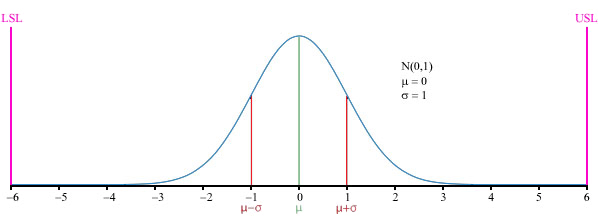
\includegraphics[width=11cm]{Abbildungen/sixs_normalverteilung}
                    \caption{Gaußsche Normalverteilung\protect\footnotemark}
                    \label{abb:normalverteilung}
                \end{center}
            \end{figure}

            \footnotetext{http://www.wikiwand.com/de/Six\_Sigma}

            Um die Abweichungen zum Zielwert möglichst gering zu halten wird der Deming-Kreis, der im ISO 9001 Kapitel vorgestellt wurde, erweitert. Six Sigma verwendet den sogenannten DMAIC Verbesserungsprozess - Define, Measure, Analyse, Improce, Control - der aus dem Kaizen Prinzip (Kai - Veränderung, Zen - Zum Besseren) aus Japan entwickelt wurde. Der DMAIC Prozess wird durchlaufen, bis die Anforderungen des Kunden erfüllt wurden.

            Zunächst wird die Problemstellung definiert. Das bedeutet, dass der Kunde befragt werden muss, welche Anforderungen er an den Prozess hat und welche Ausschuss- bzw. Fehlerrate er akzeptieren würde. Dies ist die Zielsetzung für den nachfolgenden Zyklus.

            Daraufhin wird das Maß festgelegt, an dem das Endergebnis gemessen wird. Die zuvor aufgenommenen Kundenanforderungen werden in statistische Messgrößen übersetzt und die zu messenden Kennzahlen festgelegt.
            Während eines Prozessdurchlaufs werden nun Messdaten erfasst und gespeichert.

            Die erfassten Daten werden nun analysiert und die Ursache der Abweichungen vom Zielwert wird erfasst.

            Auf Grundlage dieser Abweichungen werden Verbesserungsvorschläge erarbeitet und der Mehrwert eben dieser wird beziffert. Zu beachten ist, dass die Ursache bekämpft werden sollte und nicht die Symptome.

            Zuletzt werden Steuerungs- und Kontrollmöglichkeiten eingeführt, damit der verbesserte Prozess nachhaltig und konsistent umgesetzt wird. Das Six Sigma Team zieht sich zurück und überlässt die Kontrolle und den Prozess der ausführenden Abteilung.\footnote{Vgl. Knöfel, 2009, S. 37.} 